\chapter{Introduction}
\label{ch:intro}

This chapter introduces the motivation, background, and context for developing an \acs{FPGA} verification platform for servo drive control boards. It offers an overview of Schneider Electric’s technological environment, the function of servomechanisms, the design of the servo drive control board, and the limitations inherent in the current verification process.

\section{Motivation}
\label{sec:intro:motivation}

Modern \acs{FPGA} design and development rely on thorough verification to ensure safe, accurate, and efficient system behavior. At Schneider Electric, every new servo drive control board using an \acs{MPSoC} incorporates updated or redesigned \acs{FPGA} modules, which must be validated under realistic operating conditions before release. However, the existing verification process presents several limitations, resulting in prolonged development cycles, limited test coverage, delayed product releases, and an increased risk of critical issues remaining undetected until later stages.

To address these challenges, the company requires a dedicated \acs{FPGA} Verification Platform capable of emulating necessary inputs, automating test sequences, and enabling dynamic, repeatable, and independent verification of \acs{FPGA} modules. Such a platform would eliminate reliance on external components, offer precise control over input signals, reduce verification time, and ensure consistent test results across multiple runs.

This project seeks to modernize and enhance the \acs{FPGA} verification process by developing a flexible, scalable, and automated platform for comprehensive real-hardware testing. By treating each \acs{FPGA} module as a black box and generating precise digital and analog inputs, the platform addresses existing inefficiencies. The implementation will enable Schneider Electric to accelerate development, increase reliability, and ensure that new control boards comply with stringent performance and safety standards.

\section{Company Background}
\label{sec:intro:Company_Background}

Schneider Electric Automation GmbH is a global leader in energy management and automation. Since its founding in the 19th century, the company has expanded to offer solutions in industrial automation, building management, and sustainable energy. Its advanced servo systems enhance precision and energy efficiency in robotics, factory automation, and CNC machinery. Schneider Electric continues to play a key role in advancing servomechanism technology and robotics.

Schneider Electric’s innovations in industrial automation and robotics rely heavily on the precise control of mechanical motion. At the heart of this motion control are electric motors, which convert electric energy into mechanical energy to drive machinery. Understanding the different types of motors, they are classified as alternating current (AC) or direct current (DC) motors, depending on the type of current that generates their magnetic field \cite{Motors2024}.

\acs{AC} motors include induction motors, synchronous motors, universal motors, and switched reluctance motors. \acs{DC} motors comprise brushed \acs{DC} motors, brushless \acs{DC} motors, stepper motors, and servomotors. We are mainly interested in the Servomotors. Before that, what do we mean by “Servo” in a Servomotor? 

\subsection{Servomechanism}
\label{sec:intro:Servomechanism}

Prior to the advent of electronic systems, machinery was operated manually by individuals who shifted gears, pulled levers, or applied brakes. In contemporary settings, machinery is often controlled through buttons or knobs, with electronic circuits performing many measurements and decisions automatically. In environments where electronics and mechanical systems interact, servomechanisms are commonly employed. For example, an automobile driver monitors and controls a vehicle by making continuous adjustments to the steering wheel to maintain the vehicle's trajectory. The driver's sensory input, cognitive processing, and physical actions are analogous to the functions performed by a servomechanism. However, servomechanisms execute these tasks with greater speed, sensitivity, accuracy, and consistency. \cite{Poptronics1959}

%The fundamental principles of servo operation consist of a series of coordinated functions. Initially, the system receives instructions that specify the desired action. It then continuously monitors operating conditions and compares the current state to the intended outcome. When deviations or errors are identified, the system issues corrective commands. These commands are executed by activating the necessary mechanisms to achieve the desired performance.
\subsection{Servo Drives}
\label{sec:intro:Servo_Drives}

A servo drive, also referred to as a converter, receives control signals from controllers and regulate them to supply the required voltage and current to the servo motors. There are various types of servo drives, but the most common one is the torque-mode amplifier. This converts the command from the controller through \acs{PWM} and inverter into the specific motor current. They are mainly used for superior positioning, speed, and motion control. Servo drives are utilized in computer numerical control (CNC) machining, factory automation, robotics, and a range of other industrial applications \cite{Chhabra2019}. Figure \ref{fig:intro:servo_drive_motor} visually illustrates the essential functional relationship between the primary components: the motor, drive, and the control unit (located inside the case).

\begin{figure}[htbp]
	\centering
	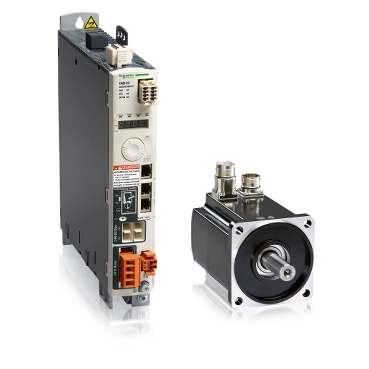
\includegraphics[width=0.45\textwidth]{gfx/diagrams/Servo_drive_and_Servo_motor_Schneider.jpg}
	\caption{Lexium 32 Servo Drive and Servo motor from Schneider Electric \cite{SchneiderElectricLexium32}}
	\label{fig:intro:servo_drive_motor}
\end{figure}

Similar to servo motors, servo drives offer a key advantage over \acs{DC} or \acs{AC} motors through the integration of motor feedbacks like current and position values. This feedback enables detection and correction of deviations from the commanded motion. Servo systems also demonstrate improved operational lifespan when maintained at constant speeds compared to conventional \acs{AC} wound motors. In industrial environments, both servo motors and servo drives are essential for monitoring position and controlling speed \cite{Chhabra2019}.

%\subsection{The Servo Drive Control Board Platform}
%\label{sec:intro:ServoDriveCBDesign}
%
%The servo drive control board under consideration (Figure \ref{fig:intro:simplified_servo_drive_control_board}) is based on the Multi-Processor System-on-Chip, which integrates application processors alongside with real-time processors. The system incorporates various hardware modules to support diverse functionalities, including motor control, signal filtering, communication interfaces, diagnostics, and debugging.
%
%\begin{figure}[H]
%	\centering
%	\begin{tikzpicture}[
%		font=\sffamily\bfseries, % Use a bold sans-serif font
%		% Define styles for consistent sizing and drawing
%		outer_square/.style={draw, very thick, minimum width=7cm, minimum height=5cm, align=center},
%		inner_square/.style={draw, thick, minimum width=5cm, minimum height=3cm, align=center, text width=2.8cm}
%		]
%		
%		% 1. Outer Square
%		% Draws the main border, centered at (0,0).
%		\node[outer_square] (outer) at (0,0) {};
%		
%		% 2. Text for the Outer Square Top (placed inside the top border)
%		\node at (outer.north) [yshift=-0.4cm] {ServoDrive Control Board};
%		
%		% 3. Inner Square with Text
%		% Draws the inner square, also centered, and holds the chip name.
%		\node[inner_square] (inner) at (0,0) {
%			MPSoC
%		};
%		
%	\end{tikzpicture}
%	\caption{Control Board Component Diagram}
%	\label{fig:intro:simplified_servo_drive_control_board}
%\end{figure}
%
%The development of a FPGA verification platform addresses the need to modernize the current design validation process. At present, most verification is performed manually, which restricts efficiency, limits dynamic testing, and introduces hardware dependencies. These challenges delay and complicate the release of new control board versions.

\section{Problem Statement}
\label{sec:intro:ProblemStatement}

In addition to standard timing and functional simulation methods for \acs{FPGA} verification, functional tests can also be conducted directly on physical hardware. Traditional RTL simulations cannot fully capture physical-layer effects or interpret bitstreams, leading to undetected bugs in reconfiguration or system integration until the design is evaluated on the actual device \cite{Gong2013}. Prior to releasing a new servo drive control board, comprehensive verification of all \acs{FPGA} modules is essential to ensure that each module meets its requirements and operates reliably within the complete hardware system.

At present, verification of servo drive control boards, particularly the \acs{FPGA} modules, is performed manually for each module. Although this method provides basic validation, it is resource-intensive, limited in scope, and unable to replicate the dynamic conditions encountered in actual operation. The process requires engineers to configure the bare-metal application in Vitis, connect the debugger, and complete multiple preparatory steps before testing can commence. Dependence on manual setup increases the likelihood of errors and prolongs the verification process. Furthermore, this approach is not easily scalable, as each test cycle must be configured and debugged individually. As \acs{FPGA} designs become more complex, the absence of automation further impedes verification efficiency and delays product release.

The existing verification method is limited to static input testing, implemented by manually assigning fixed \acs{PWM} duty cycles via \acs{AXI} registers. This confines verification to steady-state behavior and does not provide insight into servo drive performance under variable conditions such as fluctuating loads, sine-wave inputs, or abrupt disturbances. In the absence of dynamic testing, comprehensive evaluation of transient responses, control-loop stability, and the system's ability to manage unexpected changes is not feasible, potentially allowing critical issues to remain undetected.

A further limitation is the requirement for physical motors and additional hardware to generate realistic feedback signals. Measuring current on the motor phase using \acs{ADC}s requires dedicated hardware components, which increases costs and introduces variability due to hardware wear or changing environmental conditions. Additionally, this dependency complicates the testing of extreme or hazardous scenarios that cannot be safely replicated with actual motors. These constraints reduce the completeness and repeatability of the verification process.

Current measurement techniques are also inefficient, as they rely on manual estimation and on converting \acs{PWM} duty-cycle values to current levels using motor parameters. These procedures are time-consuming and must be repeated for each test cycle. The absence of automated digital tools, such as \acs{FFT}-based analysis, prevents improvements in speed, accuracy, and error detection.

An additional challenge of the present approach is the inability to test \acs{FPGA} modules independently. For instance, verifying the current-sense module requires the \acs{PWM} module to be operational in order to drive the motor and generate measurable current. This interdependence prevents isolated verification of individual modules and may obscure integration issues until late in the development process. The absence of modular testing reduces the effectiveness of incremental verification, increases risk, and can result in costly redesigns or field failures. Collectively, these challenges underscore the necessity for a more automated, flexible, and comprehensive \acs{FPGA} verification methodology for servo-drive control boards.

\section{Desired Outcome}
\label{sec:intro:DesiredOutcome}

The servo drive control board under consideration (Figure \ref{fig:intro:simplified_servo_drive_control_board}) is based on the Multi-Processor System-on-Chip, which integrates application processors alongside with real-time processors. The system incorporates various hardware modules to support diverse functionalities, including motor control, signal filtering, communication interfaces, diagnostics, and debugging.

\begin{figure}[htbp]
	\centering
	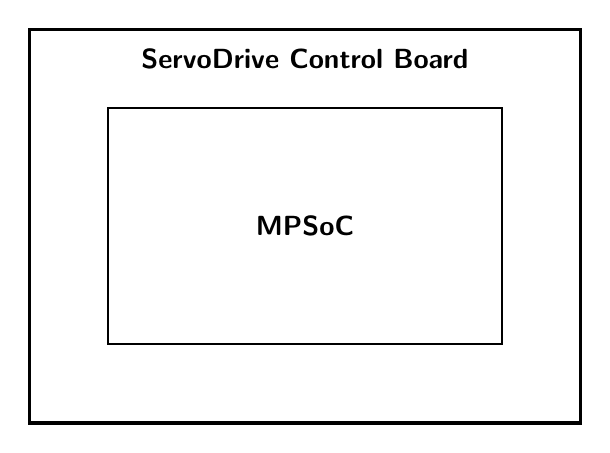
\begin{tikzpicture}[
		font=\sffamily\bfseries, % Use a bold sans-serif font
		% Define styles for consistent sizing and drawing
		outer_square/.style={draw, very thick, minimum width=7cm, minimum height=5cm, align=center},
		inner_square/.style={draw, thick, minimum width=5cm, minimum height=3cm, align=center, text width=2.8cm}
		]
		
		% 1. Outer Square
		% Draws the main border, centered at (0,0).
		\node[outer_square] (outer) at (0,0) {};
		
		% 2. Text for the Outer Square Top (placed inside the top border)
		\node at (outer.north) [yshift=-0.4cm] {ServoDrive Control Board};
		
		% 3. Inner Square with Text
		% Draws the inner square, also centered, and holds the chip name.
		\node[inner_square] (inner) at (0,0) {
			\acs{MPSoC}
		};
		
	\end{tikzpicture}
	\caption{Control Board Component Diagram}
	\label{fig:intro:simplified_servo_drive_control_board}
\end{figure}

%The development of a FPGA verification platform addresses the need to modernize the current design validation process. At present, most verification is performed manually, which restricts efficiency, limits dynamic testing, and introduces hardware dependencies. These challenges delay and complicate the release of new control board versions.

The primary objective of this project is to develop a robust proof-of-concept for a dedicated \acs{FPGA} Verification Platform. This platform will enable comprehensive verification and testing of \acs{FPGA} modules for the control board by emulating required inputs and triggers and verifying module outputs against expected behavior. As a result, the platform will substantially enhance test coverage compared to the simulation-based methodologies. This approach directly addresses the limitations identified in the previous section.

The proposed platform will automate the verification workflow, reducing or eliminating manual intervention and significantly accelerating the test cycle. It will support both static and dynamic test scenarios, enabling more exhaustive functional assessment under conditions representative of real-world operation. A key benefit is the ability to test individual modules independently of other \acs{FPGA} components or external hardware, which simplifies debugging and improves the reliability of module-level verification. The system will incorporate mechanisms for processing complex data and delivering clear, actionable results, thereby eliminating reliance on slow, error-prone manual analysis. Additionally, the platform will be designed for scalability, ensuring compatibility with various \acs{FPGA} versions of the control board and accommodating new test cases as design requirements evolve. By integrating these capabilities into a structured, intuitive workflow, the platform will deliver a significantly improved user experience compared to existing verification practices and a more efficient, reliable, and future-oriented verification methodology.
	
%\section{Starting Point}	
%\label{sec:intro:StartingPoint}
%
%\begin{figure}[H]
%	\centering
%	
\includegraphics[width=0.85\textwidth]{gfx/diagrams/Starting_Point_Thesis_Report.png}
%	\caption{FPGA Verification Test Setup} %\cite{SchneiderElectricLexium32}}
%\label{fig:intro:staring_point}
%\end{figure}
%
%The servo drive control board features a Zynq Ultrascale+ MPSoC, which incorporates a dual-core ARM Cortex-A53 application processor and a dual-core ARM Cortex-R5 real-time processor \cite{AMD2024}. This configuration enables support for applications requiring both high-performance processing and real-time control, including industrial motor control and sensor fusion.
%
%
%For the initial proof of concept, an FPGA from the same device family is selected using Enclustra hardware. As shown in the figure \ref{fig:intro:staring_point}, the setup consists of the Enclustra Mercury+ XU System-on-Module (SoM), which integrates a Xilinx Zynq UltraScale+ MPSoC, mounted on the Mercury PE1 carrier board. This board is designed to emulate the input stimuli for the design under test (DUT), specifically the target FPGA modules. The outputs generated by the DUT will be fed back to the Enclustra SoM, where they will be verified and compared against the expected reference results.
%
%The effective implementation of this verification platform depends on the advanced capabilities of the underlying System-on-Chip technology. The following chapter presents a comprehensive technical overview of the Zynq UltraScale+ MPSoC, essential clocking strategies, and relevant verification methodologies to clarify the architecture and flexibility utilized in this project.

